\documentclass{article}
\usepackage[utf8]{inputenc}
\usepackage{amsmath}
\usepackage{amsfonts}
\usepackage[margin=0.7in]{geometry}
\usepackage{graphicx}
\usepackage{amssymb}
\usepackage{gensymb}
\usepackage{booktabs}
\usepackage{wrapfig}
\usepackage{caption}
\usepackage[export]{adjustbox}
\usepackage[pdfborder={0 0 0}]{hyperref}
\usepackage{pdfpages}
\usepackage{fancyhdr}
\usepackage{parskip}
\usepackage{lastpage}
\usepackage{listings}
\usepackage{multirow}
\usepackage{xifthen}
\usepackage{xcolor}
\usepackage{mathtools}
\graphicspath{{images/}}
\pagestyle{fancy}

\begin{document}
\title{ØkIntro Aflevering 4}
\author{Carl-Emil Rohde - kvb125}
\date{Januar 2023}
\maketitle

\section*{Opgave 1}
\subsection*{1.1}
Bruttonationalprodukt (BNP) er en måling af den samlede værdi af alle goder og tjenester, der produceres inden for et land i løbet af et år. Det er en vigtig økonomisk indikator, der bruges til at måle økonomisk aktivitet og vækst. BNP kan måles på to måder, nemlig værditilskrivningsmetoden og indkomstmetoden. Værditilskrivningsmetoden er den mest almindelige og måler den samlede værdi af goder og tjenester produceret af virksomhederne i landet, mens indkomstmetoden måler den samlede indkomst genereret af arbejdere og ejere af fast ejendom i landet.

Nettonationalprodukt (NNP) er lig med BNP minus afskrivninger på fast ejendom. NNP tager højde for de omkostninger, der er forbundet med at erhverve og vedligeholde fast ejendom, såsom maskiner, bygninger og infrastruktur, som anvendes i produktionen. NNP giver derfor et mere præcist billede af den reelle vækst i økonomien, da det tager højde for erhvervelsen af fast ejendom, der kan anvendes i fremtidig produktion.

NNP er altså en mere nøjagtig måling af økonomisk vækst, da det tager højde for de investeringer der er gjort i fast ejendom. BNP er mere et mål for den samlede produktion i et land, NNP er et mål for økonomisk vækst.

\subsection*{1.2}
Pension regnes ikke med i bruttonationalproduktet (BNP), fordi pension ikke er en produktionsaktivitet. BNP måler den samlede værdi af alle goder og tjenester, der produceres i et land på et kalenderår, og her falder pension ikke ind under. Pension er i stedet en form for social sikring, hvor personer, der har arbejdet og betalt skat i et land, modtager en regelmæssig udbetaling fra det offentlige efter deres pensionsalder.

Pensionsudbetalingerne er finansieret af skatter og bidrag, som er blevet betalt i løbet af en borgers arbejdstid, og som derfor allerede er regnet med i BNP. At regne pensionsudbetalingerne med i BNP ville betyde, at regne den samme indkomst to gange. Derfor regnes pension ikke med i BNP.

\subsection*{1.3}
Der er to måder at sammenligne bruttonationalprodukt (BNP) mellem lande: BNP per capita og BNP (PPP) per capita.

BNP per capita er den gennemsnitlige værdi af BNP for hver person i et land. Dette giver et billede af den økonomiske velstand i et land i forhold til befolkningen. En højere BNP per capita indikerer typisk en højere levestandard. BNP per capita kan således være påvirket af befolkningens størrelse og aldersfordeling.

BNP (PPP) per capita er en måde at sammenligne BNP mellem lande, hvor BNP per capita korrigeres for prisniveauet i hvert land. PPP står for "purchasing power parity", som er en metode til at sammenligne den relative købekraft i forskellige lande. PPP-metoden antager, at en bestemt mængde penge kan købe den samme mængde varer og tjenester i alle lande. BNP (PPP) per capita giver altså et mere præcist billede af den relative velstand i i et land, da det tager højde for de forskellige priser på varer og tjenester.

Så kort sagt, BNP per capita giver et billede af økonomisk velstand i forhold til befolkningen, mens BNP (PPP) per capita tager højde for prisniveauet i landene og giver et mere præcist billede af den relative velstand i forskellige lande.

\section*{Opgave 2}
\subsection*{2.1}
Argentina og Chile udgør tilsammen en lukket økonomi. Derfor gælder der, at de aggregerede investeringer er lig med opsparignerne i de to lande: $I^A+I^C=A+a r+S^C$
For at finde ligevægtsrenten, isoleres $r$:
\begin{equation}
    I^A+I^C=A+a r+S^C
\end{equation}
\begin{equation}
    I^A+I^C-A-S^C=a r
\end{equation}
\begin{equation}
    r=\frac{I^A+I^C-A-S^C}{a}
\end{equation}
Således har jeg fundet et udtryk for den rente, som skaber en ligevægt mellem opsparinger og investeringer i Chile og Argentina. 

\subsection*{2.2}
Argentina og Chile's nettoeksport, er givet ved forskellen mellem de to landes opsaring og aggregerede investeringer.
\\
Argentina nettoeksport:
\begin{equation}
    N X^A=S^A-I^A=S^A-(A-a r)
\end{equation}
Chile nettoeksport:
\begin{equation}
    N X^C=S^C-I^C=S^C-(C-c r)
\end{equation}
Hvis Argentina skal være nettoeksportør, skal der naturligvis fra ligningen skrevet ovenover, gælde følgende:
\begin{equation}
    S^A>I^A=S^A>A-a r \Leftrightarrow \frac{A-S^A}{a}<r
\end{equation}
Da der i denne økonomi kun er to lande, må det betyde, at hvis Argentina skal være nettoeksportør, må Chile være nettoimporttør. Derfor må følgende gælde:
\begin{equation}
    I^C>S^C=C-c r>S^C \Leftrightarrow r<\frac{C-S^C}{c}
\end{equation}
Betingelsen for at Argentina er nettoeksportør, kan nu opskrives som følgende:
\begin{equation}
    \frac{A-S^A}{a}<r<\frac{C-S^C}{c}
\end{equation}

\section*{Opgave 3}
\subsection*{3.1}
Udtrykket for $C(Y-T)$ foreskriver, at forbrug er afhængig af disponibel indkomst, det vil sige $BNP - skat$. Det fremgår også, at $C_0$ udtrykker, at en andel af forbruget ikke afhænger af disponibel indkomst. Her er der tale om "Autonomous consumption", som er udgifter forbrugere kan have, selv hvis de ingen indkomst har. Det kunne for eksempel være mad. $C_0$ er ligeledes skæringen med y-aksen, når $C_1*(Y-T) = 0$, det vil sige når disponibel indkomst er lig 0, og dermed det forbrug der stadig er i samfundet, selvom der ikke er en disponibel indkomst. Som det antages i opgaven, giver det mening at $C_1$ er en værdi mellem 0 og 1, da det er den andel af stigningen i disponibel indkomst, som bliver brugt på forbrug. $C_1$ er altså forbrugets vækst, som funktion af den disponible indkomst. 

\subsection*{3.2}
På lang sigt må der gælde, at de planlagte udgifter svarer til BNP, altså $Y=T$. Jeg indsætter nu udtrykkene for $C(Y-T)$ og $I(r)$, og isolerer for $Y$:
\begin{equation}
    Y=C_0+C_1(Y-T)+G+I_0-I_1 r
\end{equation}
\begin{equation}
    Y=C_0+C_1 Y-C_1 T+G+I_0-I_1 r
\end{equation}
\begin{equation}
    Y-C_1 Y=C_0-C_1 T+G+I_0-I_1 r
\end{equation}
\begin{equation}
    Y\left(1-C_1\right)=C_0-C_1 T+G+I_0-I_1 r
\end{equation}
\begin{equation}
    Y(r, G, T)=\frac{C_0-C_1 T+G+I_0-I_1 r}{1-C_1}
\end{equation}
Dermed har jeg fundet et udtryk for $Y$ som funktion af $r, G$ og $T$

\subsection*{3.3}
Jeg starter med at udregne $\frac{\partial Y}{\partial G}$:
\begin{equation}
    \frac{\partial Y}{\partial G}=\frac{1}{1-C_1}
\end{equation}
Den matematisk forklaring på, at denne multiplikator er større end 1, er at $\frac{1}{1-C_1}$ altid vil være positivt under antagelse af at $0<C_1<1$, som argumenteret for i opgave 3.1. Den økonomiske forklaring på dette, er at når staten igennem forbrug øger BNP, så vil stigningen i BNP som minimum svare til det beløb de har forbrugt, og ofte mere. Stigningen i hustandenes disponible indkomst som følge af øget offentligt forbrug, medfører en stigning i privatforbrug. Dette privatforbrug resulterer i mere privatforbrug et andet sted, osv osv.. og hvis alle disse ændringer i privatforbrug lægges sammen, får man at ændringen i BNP er større end 1.

\subsection*{3.4}
Jeg starter med at udregne $\frac{\partial Y}{\partial T}$:
\begin{equation}
    \frac{\partial Y}{\partial T}=\frac{-C_1}{1-C_1}
\end{equation}
Den absolutte værdi af multiplikatoren mht T, er mindre end mht til G, da en ændring som følge af fx en skattelettelse, modsat øget privatforbrug, handler mere om hvor meget de enkelte forbrugere i forvejen havde tænkt sig at forbruge. Nogle borgere vil altså vælge bare at spare pengene op, og dermed vil pengene ikke have samme effekt når det kommer til en øgelse i BNP, som øget offentligt forbug vil. Da $0<C_1<1$, vil følgende derfor altid gælde:
\begin{equation}
    \left|\frac{-C_1}{1-C_1}\right|<\left|\frac{1}{1-C_1}\right|
\end{equation}

\subsection*{3.5}
$M_1$ er positiv, da en stigning i BNP, medfører en stigning i efterspørgsel på penge. $M_2$ er positiv, da en forøgelse af renten $r$, medfører et fald i efterspørgslen på penge. Dette kaldes ændringer i likviditetsefterpsørgslen. 

\subsection*{3.6}
Under antagelse af at der er ligevægt i markedet, sætter jeg efterspørgslen af penge, lig med udbuddet af penge og løser for $Y$:
\begin{equation}
    \frac{M}{P}=M_0+M_1 Y-M_2 r
\end{equation}
\begin{equation}
    \frac{M}{P}+M_2 r-M_0=M_1 Y
\end{equation}
\begin{equation}
    Y\left(r, \frac{M}{P}\right)=\frac{\frac{M}{P}+M_2 r-M_0}{M_1}
\end{equation}
Jeg har dermed udledt en funktion for LM-kurven.

\subsection*{3.7}
Nedenfor, har jeg indtegnet graferne for $LM$ og $IS$ kurverne med passende eksogene variable, så figuren er retvisende. IS-kurven har en negativ hældning, da en højere rente, medfører et fald i mængden af investeringer. 
\\
\\
LM-kurven har en positiv hældning, da en stigning i indkomst, har en positiv indvirkning på efterspørgslen af penge. For at udligne denne effekt, må renten også stige, og heraf den positive hældningskoefficient. 
\begin{center}
    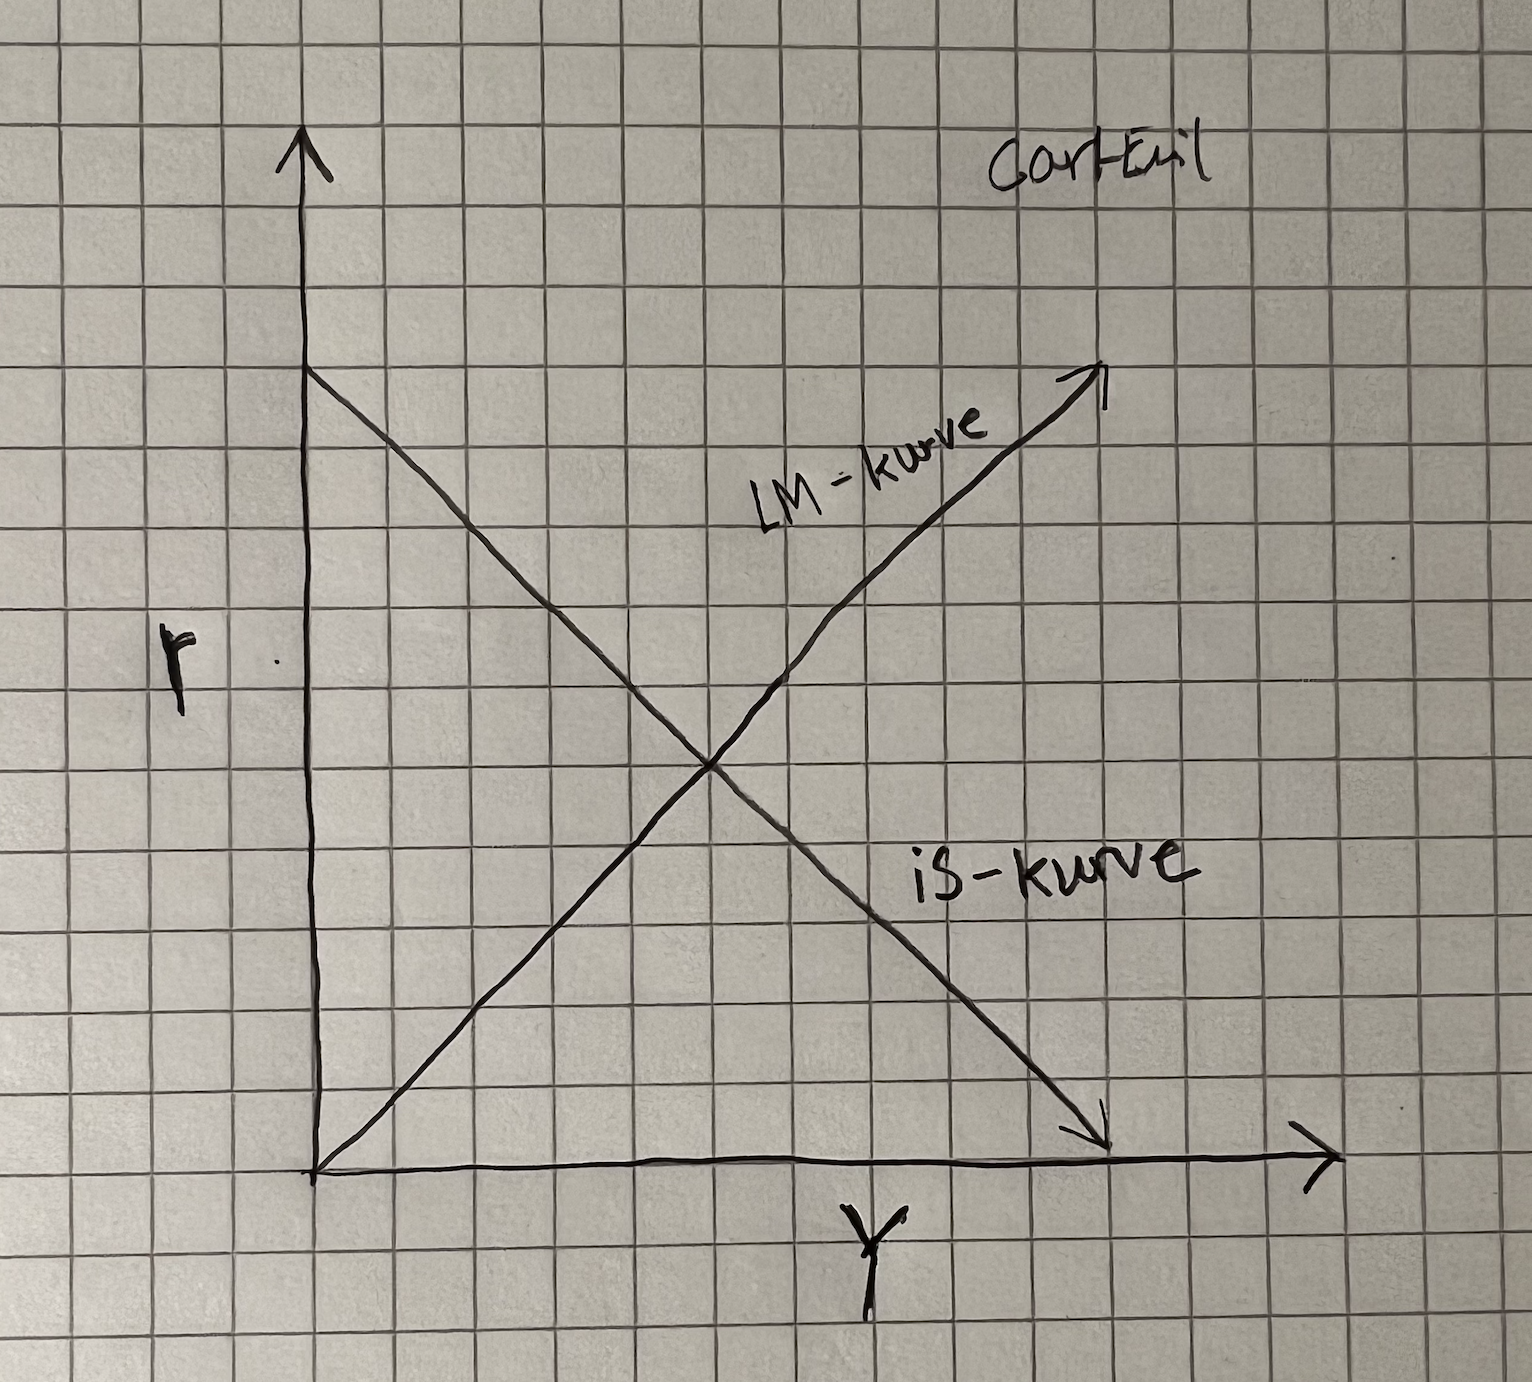
\includegraphics[scale=0.50]{w.png}
\end{center}

\subsection*{3.8}
Jeg starter med at isolere renten i udtrykket for LM-kurven:
\begin{equation}
    \frac{M}{P}=M_0+M_1 Y-M_2 r
\end{equation}
\begin{equation}
    \frac{M}{P}-M_0-M_1 Y=-M_2 r
\end{equation}
\begin{equation}
    r = \frac{-\frac{M}{P}+M_0+M_1 Y}{M_2}
\end{equation}
Dette udtryk for $r$, indsætter jeg nu i udtrykket for IS-kurven:
\begin{equation}
    Y(r, G, T)=\frac{C_0-C_1 T+G+I_0-I_1 \frac{-\frac{M}{P}+M_0+M_1 Y}{M_2}}{1-C_1}
\end{equation}
Og isolerer for $Y$:
\begin{equation}
    Y=\frac{C_0-C_1 T+G+I_0+\frac{\frac{I_1 M}{P}}{M_2}-\frac{I_1 M_0}{M_2}-\frac{I_1 M_1 Y}{M_2}}{1-C_1} \Leftrightarrow
\end{equation}
\begin{equation}
    Y=\frac{C_0-C_1 T+G+I_0+\frac{\frac{I_1 M}{P}}{M_2}-\frac{I_1 M_0}{M_2}}{1-C_1}-\frac{\frac{I_1 M_1 Y}{M_2}}{1-C_1} \Leftrightarrow
\end{equation}
\begin{equation}
    Y+\frac{\frac{I_1 M_1 Y}{M_2}}{1-C_1}=\frac{C_0-C_1 T+G+I_0+\frac{\frac{I_1 M}{P}}{M_2}-\frac{I_1 M_0}{M_2}}{1-C_1} \Leftrightarrow
\end{equation}
\begin{equation}
    Y\left(1-C_1+\frac{I_1 M_1}{M_2}\right)=C_0-C_1 T+G+I_0+\frac{\frac{I_1 M}{P}}{M_2}-\frac{I_1 M_0}{M_2} \Leftrightarrow
\end{equation}
\begin{equation}
    Y=\frac{C_0-C_1 T+G+I_0+\frac{\frac{I_1 M}{P}}{M_2}-\frac{I_1 M_0}{M_2}}{1-C_1+\frac{I_1 M_1}{M_2}}
\end{equation}
Jeg har dermed fundet et udtryk for BNP i ligevægt. 

\subsection*{3.9}
Jeg starter med at udregne $\frac{\partial Y}{\partial G}$:
\begin{equation}
    \frac{\partial Y}{\partial G}=\frac{1}{\frac{I_1 M_1}{M_2}+1-C_1}
\end{equation}
Sammenlignes dette resultat med udtrykket fra opgave 3.3, ser vi at:
\begin{equation}
    \frac{1}{\frac{I_1 M_1}{M_2}+1-C_1}<\frac{1}{1-C_1}
\end{equation}
da det er givet at $I_1, M_1, M_2>0$.
\\
\\
Når man undersøger IS-kurven, kan man se at en øgning i offentligt forbrug resulterer i et fald i renten. På den anden side, hvis man kun kigger på LM-kurven, kan man se at en øgning i offentligt forbrug fører til en stigning i renten. Disse to scenarier har modstridende effekter, og derfor vil BNP øges mere, hvis man kun ser på IS-kurven, da BNP i ligevægt afhænger både af IS- og LM-kurven.

\subsection*{3.10}
Jeg starter med at isolere $M$ i udtrykket fra opgave 3.8 (ligning 23):
\begin{equation}
    Y=\frac{C_0-C_1 T+G+I_0-I_1 \frac{-\frac{M}{P}+M_0+M_1 Y}{M_2}}{1-C_1}
\end{equation}
\begin{equation}
    \frac{\frac{I_1 \frac{-M}{P}}{M_2}}{1-C_1}=Y-\frac{C_0-C_1 T+G+I_0-I_1 \frac{M_0+M_1 Y}{M_2}}{1-C_1}
\end{equation}
\begin{equation}
    I_1 \frac{-M}{P}=\frac{M_2 Y}{1-C_1}-M_2\left(C_0-C_1 T+G+I_0-I_1 \frac{M_0+M_1 Y}{M_2}\right)
\end{equation}
\begin{equation}
    M=-P \frac{\frac{M_2 Y}{1-C_1}-M_2\left(C_0-C_1 T+G+I_0-I_1 \frac{M_0+M_1 Y}{M_2}\right)}{I_1}
\end{equation}
Finder $\frac{\partial M}{\partial C_0}$:
\begin{equation}
    \frac{\partial M}{\partial C_0}=-\frac{P M_2}{I_1}
\end{equation}
Der er en positiv sammenhæng mellem pengemængden og BNP, så hvis BNP er uændret, kan man sige, at centralbanken skal øge pengemængden med $\frac{P M_2}{I_1}$, for hver enhed $C_0$ falder. Dette er dog en stærkt simplificeret model. I virkeligheden kan centralbanken ikke kompensere for fald i $C_0$ ved at øge pengemængden alene.





\end{document}
